\documentclass[a4paper,12pt]{article}
\usepackage{fontspec}
\setmainfont{Noto Serif CJK JP}[Scale=1.0]
\usepackage{amsmath,amssymb,amsthm}
\usepackage{tikz-cd}
\usepackage{tikz}
\usetikzlibrary{positioning,shapes,arrows,decorations.pathmorphing,calc,patterns}
\usepackage{hyperref}
\usepackage[margin=25mm]{geometry}
\usepackage{listings}
\usepackage{xcolor}

\theoremstyle{definition}
\newtheorem{definition}{定義}[section]
\newtheorem{theorem}[definition]{定理}
\newtheorem{lemma}[definition]{補題}
\newtheorem{proposition}[definition]{命題}
\newtheorem{example}[definition]{例}
\newtheorem{remark}[definition]{注意}
\newtheorem{corollary}[definition]{系}

\lstdefinestyle{leanstyle}{
  basicstyle=\ttfamily\small,
  keywordstyle=\color{blue}\bfseries,
  commentstyle=\color{green!60!black},
  stringstyle=\color{red},
  showstringspaces=false,
  breaklines=true,
  frame=single,
  numbers=left,
  numberstyle=\tiny\color{gray}
}

\title{自然数の構造塔\\
\large 忘却関手の具体例による理解}
\author{Claude (Anthropic) によるTeX生成\\CODEX (OpenAI) によるLean形式化}
\date{\today}

\begin{document}

\maketitle

\begin{abstract}
本稿では、抽象的な構造塔理論を自然数という具体的な例を通じて理解する。自然数$\mathbb{N}$上に構造塔を構成し、後者関数(successor function)が誘導する射を詳しく調べる。さらに、忘却関手がこれらの具体的な構造にどのように作用するかを明示的に計算する。Lean 4による形式化を通じて、抽象的な圏論の概念が具体的な数学的対象にどのように適用されるかを学ぶ。
\end{abstract}

\tableofcontents

\section{導入}

\subsection{これまでの流れ}

これまでに学んできた概念:
\begin{enumerate}
\item 構造塔: 順序に従って単調増大する集合の族
\item 最小層付き構造塔: 各要素が初めて現れる層を明示
\item 構造塔の射: 構造を保つ写像
\item 構造塔の圏: 構造塔全体が形成する圏
\item 忘却関手: 構造を「忘れる」関手
\end{enumerate}

\subsection{本稿の目的}

本稿では、これらの抽象的な概念を\textbf{自然数}という最も基本的な数学的対象を通じて具体的に理解する。以下を達成する:

\begin{itemize}
\item 自然数上の構造塔$\mathbb{N}\text{-Tower}$の明示的な構成
\item 後者関数$\text{succ} : n \mapsto n+1$が誘導する射の性質
\item 忘却関手による射の像の計算
\item 抽象理論と具体例の対応関係の理解
\end{itemize}

\section{自然数の構造塔}

\subsection{直観的説明}

自然数$\mathbb{N} = \{0, 1, 2, 3, \ldots\}$上に、次のような階層構造を考える:
\begin{align*}
\text{Layer } 0 &= \{0\} \\
\text{Layer } 1 &= \{0, 1\} \\
\text{Layer } 2 &= \{0, 1, 2\} \\
\text{Layer } 3 &= \{0, 1, 2, 3\} \\
&\vdots
\end{align*}

各層は「$n$以下の自然数全体」を表している。

\subsection{視覚化}

自然数の構造塔を図示すると以下のようになる:

\begin{center}
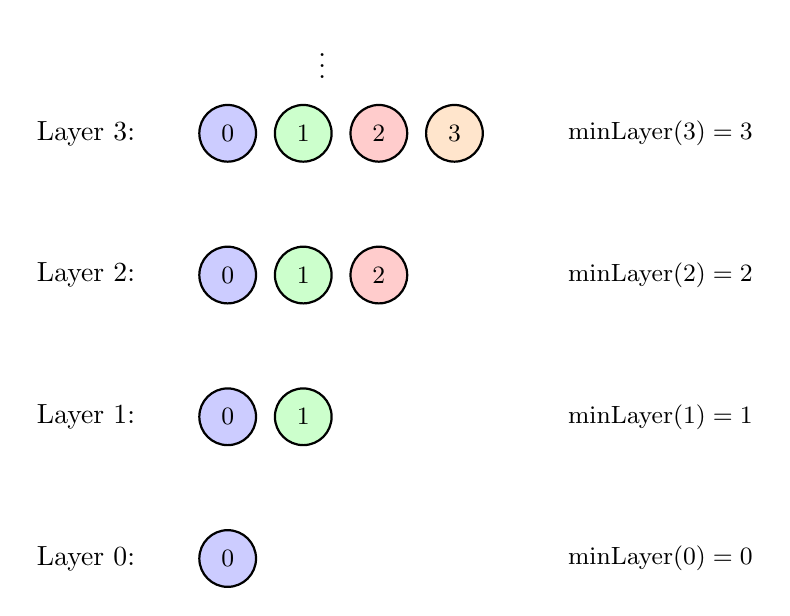
\begin{tikzpicture}[scale=1.2]
% Layer 0
\draw[thick, fill=blue!20] (0,0) circle (0.3);
\node at (0,0) {\small $0$};
\node at (-1.5,0) {Layer 0:};

% Layer 1
\draw[thick, fill=blue!20] (0,1.5) circle (0.3);
\node at (0,1.5) {\small $0$};
\draw[thick, fill=green!20] (0.8,1.5) circle (0.3);
\node at (0.8,1.5) {\small $1$};
\node at (-1.5,1.5) {Layer 1:};

% Layer 2
\draw[thick, fill=blue!20] (0,3) circle (0.3);
\node at (0,3) {\small $0$};
\draw[thick, fill=green!20] (0.8,3) circle (0.3);
\node at (0.8,3) {\small $1$};
\draw[thick, fill=red!20] (1.6,3) circle (0.3);
\node at (1.6,3) {\small $2$};
\node at (-1.5,3) {Layer 2:};

% Layer 3
\draw[thick, fill=blue!20] (0,4.5) circle (0.3);
\node at (0,4.5) {\small $0$};
\draw[thick, fill=green!20] (0.8,4.5) circle (0.3);
\node at (0.8,4.5) {\small $1$};
\draw[thick, fill=red!20] (1.6,4.5) circle (0.3);
\node at (1.6,4.5) {\small $2$};
\draw[thick, fill=orange!20] (2.4,4.5) circle (0.3);
\node at (2.4,4.5) {\small $3$};
\node at (-1.5,4.5) {Layer 3:};

\node at (1,5.3) {$\vdots$};

% 凡例
\node[anchor=west] at (3.5,0) {\small $\text{minLayer}(0) = 0$};
\node[anchor=west] at (3.5,1.5) {\small $\text{minLayer}(1) = 1$};
\node[anchor=west] at (3.5,3) {\small $\text{minLayer}(2) = 2$};
\node[anchor=west] at (3.5,4.5) {\small $\text{minLayer}(3) = 3$};
\end{tikzpicture}
\end{center}

各自然数$n$は、レイヤー$n$で初めて現れる（色分けで表示）。

\subsection{形式的定義}

\begin{definition}[自然数の構造塔]\label{def:nat_tower}
自然数の構造塔$\mathbb{N}\text{-Tower}$を以下で定義する:
\begin{itemize}
\item 台集合: $\text{carrier} = \mathbb{N}$
\item 添字集合: $\text{Index} = \mathbb{N}$ (通常の順序$\leq$)
\item 層関数: $\text{layer}(n) := \{k \in \mathbb{N} \mid k \leq n\}$
\item 最小層関数: $\text{minLayer}(n) := n$ (恒等関数)
\end{itemize}
\end{definition}

\begin{proposition}[構造塔の条件]
定義\ref{def:nat_tower}の$\mathbb{N}\text{-Tower}$は、最小層付き構造塔の全ての条件を満たす。
\end{proposition}

\begin{proof}
以下の5つの条件を確認する。

\paragraph{(1) 被覆条件}
任意の$x \in \mathbb{N}$に対して、$i = x$とすれば、$x \leq x$より$x \in \text{layer}(x)$である。

\paragraph{(2) 単調性}
$i \leq j$とする。$x \in \text{layer}(i)$ならば$x \leq i$である。$i \leq j$より$x \leq j$、したがって$x \in \text{layer}(j)$。よって$\text{layer}(i) \subseteq \text{layer}(j)$。

\paragraph{(3) 最小層の所属性}
任意の$x \in \mathbb{N}$に対して、$\text{minLayer}(x) = x$である。$x \leq x$より、$x \in \text{layer}(x) = \text{layer}(\text{minLayer}(x))$。

\paragraph{(4) 最小層の最小性}
$x \in \text{layer}(i)$とする。これは$x \leq i$を意味する。$\text{minLayer}(x) = x$より、$\text{minLayer}(x) = x \leq i$が成立する。
\end{proof}

\subsection{Lean 4での実装}

Lean 4では以下のように実装される:

\begin{lstlisting}[style=leanstyle, language=ML]
def natTowerMin : StructureTowerWithMin.{0, 0} where
  carrier := ℕ
  Index := ℕ
  layer := fun n => {k : ℕ | k ≤ n}
  covering := by intro x; use x; exact le_refl x
  monotone := by intro i j hij x hx; exact le_trans hx hij
  minLayer := _root_.id
  minLayer_mem := by intro x; exact le_refl x
  minLayer_minimal := by intro x i hx; exact hx
\end{lstlisting}

\begin{remark}
\texttt{\{0, 0\}}は宇宙レベルを表し、$\mathbb{N}$は\texttt{Type 0}に属することを意味する。
\end{remark}

\section{後者関数が誘導する射}

\subsection{後者関数}

\begin{definition}[後者関数]
\textbf{後者関数}(successor function) $\text{succ} : \mathbb{N} \to \mathbb{N}$を次で定義する:
\[
\text{succ}(n) := n + 1
\]
\end{definition}

これは最も基本的な自然数の操作の一つである。

\subsection{射の構成}

後者関数は、$\mathbb{N}\text{-Tower}$から自分自身への射を誘導する。

\begin{theorem}[後者射]\label{thm:succ_hom}
以下のデータは、構造塔の射$f : \mathbb{N}\text{-Tower} \to \mathbb{N}\text{-Tower}$を定義する:
\begin{itemize}
\item 台写像: $f.\text{map} = \text{succ}$
\item 添字写像: $f.\text{indexMap} = \text{succ}$
\end{itemize}
\end{theorem}

\begin{proof}
射の5つの条件を確認する。

\paragraph{(1) 添字写像の単調性}
$i \leq j$とする。このとき、
\[
f.\text{indexMap}(i) = i + 1 \leq j + 1 = f.\text{indexMap}(j)
\]
これは自然数の順序の性質より明らかである。

\paragraph{(2) 層の保存性}
$x \in \text{layer}(i)$、すなわち$x \leq i$とする。このとき、
\[
f.\text{map}(x) = x + 1 \leq i + 1 = f.\text{indexMap}(i)
\]
したがって$f.\text{map}(x) \in \text{layer}(f.\text{indexMap}(i))$。

\paragraph{(3) 最小層の保存性}
任意の$x \in \mathbb{N}$に対して、
\begin{align*}
\text{minLayer}(f.\text{map}(x)) &= \text{minLayer}(x + 1) \\
&= x + 1 \quad \text{(定義より)} \\
&= \text{succ}(x) \\
&= f.\text{indexMap}(\text{minLayer}(x))
\end{align*}
\end{proof}

\subsection{後者射の視覚化}

後者射は、各層を次の層へ「シフト」する:

\begin{center}
\begin{tikzcd}[row sep=large, column sep=huge]
\text{Layer } i \arrow[r, "\text{succ}"] \arrow[d, hook] 
& \text{Layer } (i+1) \arrow[d, hook] \\
\{0, 1, \ldots, i\} \arrow[r, "n \mapsto n+1"] 
& \{0, 1, \ldots, i+1\}
\end{tikzcd}
\end{center}

具体的には:
\begin{align*}
\text{succ}(\text{Layer } 0) &= \text{succ}(\{0\}) = \{1\} \subseteq \text{Layer } 1 \\
\text{succ}(\text{Layer } 1) &= \text{succ}(\{0, 1\}) = \{1, 2\} \subseteq \text{Layer } 2 \\
\text{succ}(\text{Layer } 2) &= \text{succ}(\{0, 1, 2\}) = \{1, 2, 3\} \subseteq \text{Layer } 3
\end{align*}

\subsection{Lean 4での実装}

\begin{lstlisting}[style=leanstyle, language=ML]
def natSuccHom : natTowerMin ⟶ natTowerMin where
  map := Nat.succ
  indexMap := Nat.succ
  indexMap_mono := by
    intro i j hij
    exact Nat.succ_le_succ hij
  layer_preserving := by
    intro i x hx
    show Nat.succ x ≤ Nat.succ i
    exact Nat.succ_le_succ hx
  minLayer_preserving := by intro x; rfl
\end{lstlisting}

\section{忘却関手の適用}

\subsection{台集合への忘却}

台集合への忘却関手$U_{\text{carrier}}$を後者射に適用すると何が起こるか？

\begin{proposition}[台写像の忘却]\label{prop:forget_carrier_succ}
\[
U_{\text{carrier}}(\text{natSuccHom}) = \text{succ} : \mathbb{N} \to \mathbb{N}
\]
\end{proposition}

\begin{proof}
定義より、
\begin{align*}
U_{\text{carrier}}(\text{natSuccHom}) &= (\text{natSuccHom}).\text{map} \\
&= \text{succ}
\end{align*}
\end{proof}

\begin{remark}
忘却関手は、構造塔の射から台写像だけを取り出す。この場合、$\text{succ}$という単純な関数が得られる。
\end{remark}

\subsection{添字集合への忘却}

同様に、添字集合への忘却関手を考える。

\begin{proposition}[添字写像の忘却]\label{prop:forget_index_succ}
\[
U_{\text{Index}}(\text{natSuccHom}) = \text{succ} : \mathbb{N} \to \mathbb{N}
\]
\end{proposition}

\begin{proof}
\begin{align*}
U_{\text{Index}}(\text{natSuccHom}) &= (\text{natSuccHom}).\text{indexMap} \\
&= \text{succ}
\end{align*}
\end{proof}

\begin{remark}
$\mathbb{N}\text{-Tower}$は特殊な例であり、台集合と添字集合が同じ$\mathbb{N}$である。さらに、後者射は両方の写像が同じ$\text{succ}$関数である。
\end{remark}

\subsection{可換図式}

忘却関手の作用を可換図式で表すと:

\begin{center}
\begin{tikzcd}[row sep=huge, column sep=huge]
\mathbb{N}\text{-Tower} \arrow[r, "\text{natSuccHom}"] \arrow[d, "U_{\text{carrier}}"'] 
& \mathbb{N}\text{-Tower} \arrow[d, "U_{\text{carrier}}"] \\
\mathbb{N} \arrow[r, "\text{succ}"'] 
& \mathbb{N}
\end{tikzcd}
\end{center}

また、添字についても:

\begin{center}
\begin{tikzcd}[row sep=huge, column sep=huge]
\mathbb{N}\text{-Tower} \arrow[r, "\text{natSuccHom}"] \arrow[d, "U_{\text{Index}}"'] 
& \mathbb{N}\text{-Tower} \arrow[d, "U_{\text{Index}}"] \\
\mathbb{N} \arrow[r, "\text{succ}"'] 
& \mathbb{N}
\end{tikzcd}
\end{center}

これらの図式の可換性は、命題\ref{prop:forget_carrier_succ}と\ref{prop:forget_index_succ}そのものである。

\section{恒等射と忘却関手}

\subsection{恒等射の忘却}

構造塔の恒等射$\text{id}_{\mathbb{N}\text{-Tower}}$を忘却するとどうなるか？

\begin{proposition}[恒等射の忘却]\label{prop:forget_id}
\[
U_{\text{carrier}}(\text{id}_{\mathbb{N}\text{-Tower}}) = \text{id}_{\mathbb{N}}
\]
\end{proposition}

\begin{proof}
構造塔の恒等射は、定義より$(\text{id}_{\mathbb{N}\text{-Tower}}).\text{map} = \text{id}_{\mathbb{N}}$である。したがって、
\[
U_{\text{carrier}}(\text{id}_{\mathbb{N}\text{-Tower}}) = (\text{id}_{\mathbb{N}\text{-Tower}}).\text{map} = \text{id}_{\mathbb{N}}
\]
\end{proof}

\begin{remark}
これは関手の恒等射保存性の具体例である。忘却関手$U_{\text{carrier}}$は恒等射を恒等射に写す。
\end{remark}

\subsection{Lean 4での証明}

\begin{lstlisting}[style=leanstyle, language=ML]
lemma forgetCarrier_id :
    forgetCarrier.map (𝟙 natTowerMin) = _root_.id := by
  funext x; rfl
\end{lstlisting}

ここで、\texttt{𝟙}は圏論での恒等射の記法である。

\section{射の合成と忘却関手}

\subsection{合成の保存}

関手は射の合成を保存する。これを$\mathbb{N}\text{-Tower}$で確認しよう。

\begin{theorem}[合成の保存]\label{thm:forget_comp}
任意の2つの射$f, g : \mathbb{N}\text{-Tower} \to \mathbb{N}\text{-Tower}$に対して、
\[
U_{\text{carrier}}(g \circ f) = U_{\text{carrier}}(g) \circ U_{\text{carrier}}(f)
\]
\end{theorem}

\begin{proof}
定義を展開すると:
\begin{align*}
U_{\text{carrier}}(g \circ f) &= (g \circ f).\text{map} \\
&= g.\text{map} \circ f.\text{map} \quad \text{(射の合成の定義)} \\
&= U_{\text{carrier}}(g) \circ U_{\text{carrier}}(f)
\end{align*}
\end{proof}

\subsection{具体例: 後者射の2回合成}

後者射を2回合成すると、$n \mapsto n + 2$という写像が得られる。

\begin{example}
\[
\text{natSuccHom} \circ \text{natSuccHom}
\]
を考える。忘却関手で写すと:
\begin{align*}
U_{\text{carrier}}(\text{natSuccHom} \circ \text{natSuccHom}) &= U_{\text{carrier}}(\text{natSuccHom}) \circ U_{\text{carrier}}(\text{natSuccHom}) \\
&= \text{succ} \circ \text{succ} \\
&= (n \mapsto n + 2)
\end{align*}
\end{example}

\subsection{図式による理解}

\begin{center}
\begin{tikzcd}[row sep=huge, column sep=large]
\mathbb{N}\text{-Tower} \arrow[r, "f"] \arrow[rr, bend left=20, "g \circ f"] \arrow[d, "U"'] 
& \mathbb{N}\text{-Tower} \arrow[r, "g"] \arrow[d, "U"'] 
& \mathbb{N}\text{-Tower} \arrow[d, "U"] \\
\mathbb{N} \arrow[r, "U(f)"'] \arrow[rr, bend right=20, "U(g) \circ U(f)"] 
& \mathbb{N} \arrow[r, "U(g)"'] 
& \mathbb{N}
\end{tikzcd}
\end{center}

この図式は、上の経路と下の経路が一致すること、すなわち定理\ref{thm:forget_comp}を表している。

\section{特殊な性質}

\subsection{台集合と添字集合の一致}

$\mathbb{N}\text{-Tower}$では、台集合と添字集合が両方とも$\mathbb{N}$である。

\begin{proposition}[集合の一致]
\[
U_{\text{carrier}}(\mathbb{N}\text{-Tower}) = U_{\text{Index}}(\mathbb{N}\text{-Tower}) = \mathbb{N}
\]
\end{proposition}

\begin{proof}
定義より明らか:
\begin{align*}
U_{\text{carrier}}(\mathbb{N}\text{-Tower}) &= (\mathbb{N}\text{-Tower}).\text{carrier} = \mathbb{N} \\
U_{\text{Index}}(\mathbb{N}\text{-Tower}) &= (\mathbb{N}\text{-Tower}).\text{Index} = \mathbb{N}
\end{align*}
\end{proof}

\begin{remark}
これは$\mathbb{N}\text{-Tower}$の特殊性である。一般の構造塔では、台集合と添字集合は異なる型を持つ。
\end{remark}

\subsection{自己同型としての後者射}

後者射は$\mathbb{N}\text{-Tower}$から自分自身への射(自己射、endomorphism)である。

\begin{definition}[自己射のモノイド]
構造塔$T$の自己射全体
\[
\text{End}(T) := \text{Hom}(T, T)
\]
は、射の合成を演算として\textbf{モノイド}(monoid)を形成する。
\end{definition}

\begin{proposition}
$\text{natSuccHom} \in \text{End}(\mathbb{N}\text{-Tower})$である。
\end{proposition}

\subsection{忘却関手とモノイド準同型}

\begin{theorem}[モノイド準同型]
忘却関手$U_{\text{carrier}} : \text{End}(\mathbb{N}\text{-Tower}) \to \text{End}(\mathbb{N})$は、モノイド準同型である。
\end{theorem}

\begin{proof}
以下の2つの性質を示せばよい:
\begin{enumerate}
\item 単位元の保存: $U_{\text{carrier}}(\text{id}) = \text{id}$ (命題\ref{prop:forget_id})
\item 演算の保存: $U_{\text{carrier}}(g \circ f) = U_{\text{carrier}}(g) \circ U_{\text{carrier}}(f)$ (定理\ref{thm:forget_comp})
\end{enumerate}
両方とも既に証明済みである。
\end{proof}

\section{より一般的な構造塔との比較}

\subsection{$\mathbb{N}\text{-Tower}$の特殊性}

$\mathbb{N}\text{-Tower}$は、以下の点で特殊である:

\begin{enumerate}
\item \textbf{台集合と添字集合の一致}: $\text{carrier} = \text{Index} = \mathbb{N}$
\item \textbf{最小層が恒等写像}: $\text{minLayer}(n) = n$
\item \textbf{層の明示的な形}: $\text{layer}(n) = \{0, 1, \ldots, n\}$
\item \textbf{可算性}: 台集合も添字集合も可算集合
\end{enumerate}

\subsection{一般の構造塔}

一般の構造塔では:
\begin{itemize}
\item 台集合と添字集合は異なる型
\item 最小層は複雑な関数
\item 層の形は抽象的
\item 非可算な場合もある
\end{itemize}

\subsection{対比表}

\begin{center}
\begin{tabular}{|l|l|l|}
\hline
性質 & $\mathbb{N}\text{-Tower}$ & 一般の構造塔 \\ \hline
台集合 & $\mathbb{N}$ & 任意の型$\alpha$ \\ \hline
添字集合 & $\mathbb{N}$ & 任意の前順序集合$\iota$ \\ \hline
層 & $\{k \mid k \leq n\}$ & 抽象的な部分集合 \\ \hline
最小層 & $\text{id}$ & 複雑な関数 \\ \hline
計算可能性 & 明示的に計算可能 & 一般には非計算的 \\ \hline
\end{tabular}
\end{center}

\section{忘却関手の計算例}

\subsection{例1: 恒等射}

\begin{align*}
U_{\text{carrier}}(\text{id}_{\mathbb{N}\text{-Tower}}) &= \text{id}_{\mathbb{N}} \\
&= (n \mapsto n)
\end{align*}

\subsection{例2: 後者射}

\begin{align*}
U_{\text{carrier}}(\text{natSuccHom}) &= \text{succ} \\
&= (n \mapsto n + 1)
\end{align*}

\subsection{例3: 後者射の2回合成}

\begin{align*}
U_{\text{carrier}}(\text{natSuccHom} \circ \text{natSuccHom}) &= \text{succ} \circ \text{succ} \\
&= (n \mapsto n + 2)
\end{align*}

\subsection{例4: 後者射の$k$回合成}

一般に、$k \in \mathbb{N}$に対して:
\begin{align*}
U_{\text{carrier}}(\underbrace{\text{natSuccHom} \circ \cdots \circ \text{natSuccHom}}_{k\text{回}}) &= \underbrace{\text{succ} \circ \cdots \circ \text{succ}}_{k\text{回}} \\
&= (n \mapsto n + k)
\end{align*}

\section{教育的意義}

\subsection{抽象と具体の橋渡し}

$\mathbb{N}\text{-Tower}$は、以下の理由で教育的に重要である:

\begin{enumerate}
\item \textbf{具体性}: 誰もが知っている自然数を使用
\item \textbf{計算可能性}: すべての概念が明示的に計算できる
\item \textbf{視覚化}: 層構造を図で表現しやすい
\item \textbf{直観}: 抽象的な概念の具体的なイメージを提供
\end{enumerate}

\subsection{形式化の価値}

Lean 4による形式化は:
\begin{itemize}
\item 定義が曖昧さなく記述される
\item 証明が機械的に検証される
\item 抽象理論と具体例の対応が明確になる
\item エラーや見落としが防止される
\end{itemize}

\section{発展的話題}

\subsection{他の構造塔の例}

\begin{example}[整数の構造塔]
$\mathbb{Z}$上に同様の構造塔を構成できる:
\[
\text{layer}(n) = \{k \in \mathbb{Z} \mid |k| \leq n\}
\]
\end{example}

\begin{example}[有限集合の構造塔]
有限集合$\{0, 1, \ldots, N-1\}$上の構造塔も自然に定義できる。
\end{example}

\subsection{射の圏論的性質}

\begin{definition}[射のモノイド構造]
$\text{End}(\mathbb{N}\text{-Tower})$は、以下の構造を持つ:
\begin{itemize}
\item 演算: 射の合成$\circ$
\item 単位元: 恒等射$\text{id}$
\item 結合律: $(h \circ g) \circ f = h \circ (g \circ f)$
\end{itemize}
\end{definition}

\subsection{加法との関係}

自然数の加法$+ : \mathbb{N} \times \mathbb{N} \to \mathbb{N}$と後者関数には深い関係がある:
\[
m + n = \underbrace{\text{succ}(\text{succ}(\cdots \text{succ}}_{\text{$n$回}}(m) \cdots ))
\]

これは、後者関数の反復によって加法が定義できることを示している。

\section{まとめ}

本稿では、自然数$\mathbb{N}$上の構造塔を通じて、抽象的な圏論の概念を具体的に理解した。主要な成果は以下の通りである:

\begin{itemize}
\item 自然数の構造塔$\mathbb{N}\text{-Tower}$の明示的な構成
\item 後者関数が誘導する射の詳細な解析
\item 忘却関手$U_{\text{carrier}}$と$U_{\text{Index}}$の具体的な計算
\item 恒等射の保存と合成の保存の具体例
\item モノイド準同型としての忘却関手の理解
\end{itemize}

$\mathbb{N}\text{-Tower}$は特殊な例であるが、その単純さゆえに、抽象的な理論の本質を理解する上で非常に有用である。抽象理論を学ぶ際には、このような具体例を常に念頭に置くことで、直観と形式的理解の両方を深めることができる。

Lean 4による形式化は、これらの概念を機械的に検証可能な形で記述し、数学の厳密性を保証する強力な手段である。

\section*{参考文献}

\begin{enumerate}
\item Saunders Mac Lane, \textit{Categories for the Working Mathematician}, Springer, 1971.
\item Tom Leinster, \textit{Basic Category Theory}, Cambridge University Press, 2014.
\item The mathlib Community, \textit{The Lean Mathematical Library}, \url{https://github.com/leanprover-community/mathlib4}
\item N. Bourbaki, \textit{Elements of Mathematics: Theory of Sets}, Springer, 2004.
\item Edmund Landau, \textit{Foundations of Analysis}, Chelsea Publishing, 1951.
\end{enumerate}

\appendix

\section{Lean 4コードの全文}

本稿で解説した自然数の構造塔と忘却関手の形式化の全体は以下の通りである:

\begin{lstlisting}[style=leanstyle, language=ML]
import Mathlib.Data.Set.Basic
import Mathlib.Order.Basic
import Mathlib.CategoryTheory.Category.Basic
import Mathlib.CategoryTheory.Functor.Basic
import Mathlib.CategoryTheory.Types.Basic

universe u v

structure StructureTowerWithMin where
  carrier : Type u
  Index : Type v
  [indexPreorder : Preorder Index]
  layer : Index → Set carrier
  covering : ∀ x : carrier, ∃ i : Index, x ∈ layer i
  monotone : ∀ {i j : Index}, i ≤ j → layer i ⊆ layer j
  minLayer : carrier → Index
  minLayer_mem : ∀ x, x ∈ layer (minLayer x)
  minLayer_minimal : ∀ {x i}, x ∈ layer i → minLayer x ≤ i

namespace StructureTowerWithMin

-- (構造塔の基本定義は省略)

def natTowerMin : StructureTowerWithMin.{0, 0} where
  carrier := ℕ
  Index := ℕ
  layer := fun n => {k : ℕ | k ≤ n}
  covering := by intro x; use x; exact le_refl x
  monotone := by intro i j hij x hx; exact le_trans hx hij
  minLayer := _root_.id
  minLayer_mem := by intro x; exact le_refl x
  minLayer_minimal := by intro x i hx; exact hx

def natSuccHom : natTowerMin ⟶ natTowerMin where
  map := Nat.succ
  indexMap := Nat.succ
  indexMap_mono := by
    intro i j hij
    exact Nat.succ_le_succ hij
  layer_preserving := by
    intro i x hx
    show Nat.succ x ≤ Nat.succ i
    exact Nat.succ_le_succ hx
  minLayer_preserving := by intro x; rfl

lemma forgetCarrier_natSuccHom :
    forgetCarrier.map natSuccHom = Nat.succ := by
  funext x; rfl

lemma forgetIndex_natSuccHom :
    forgetIndex.map natSuccHom = Nat.succ := by
  funext i; rfl

lemma forgetCarrier_id :
    forgetCarrier.map (𝟙 natTowerMin) = _root_.id := by
  funext x; rfl

lemma forgetCarrier_comp (f g : natTowerMin ⟶ natTowerMin) :
    forgetCarrier.map (f ≫ g) = 
    forgetCarrier.map f ≫ forgetCarrier.map g := by
  rfl

example : forgetCarrier.obj natTowerMin = ℕ := rfl
example : forgetIndex.obj natTowerMin = ℕ := rfl

lemma natTower_carrier_eq_index :
    forgetCarrier.obj natTowerMin = 
    forgetIndex.obj natTowerMin := rfl

end StructureTowerWithMin
\end{lstlisting}

\section{演習問題}

\begin{enumerate}
\item $\mathbb{N}\text{-Tower}$において、層$\text{layer}(5)$の要素をすべて列挙せよ。

\item 後者射を3回合成した$\text{natSuccHom}^3$を忘却関手で写すと、どのような関数が得られるか計算せよ。

\item $\mathbb{Z}$上の構造塔を定義し、その最小層関数を求めよ。

\item $\mathbb{N}\text{-Tower}$において、$\text{layer}(i) \cap \text{layer}(j) = \text{layer}(\min(i, j))$が成立することを示せ。

\item 後者射$\text{natSuccHom}$が全射でない理由を説明せよ。

\item 一般の構造塔で台集合と添字集合が一致する必要十分条件を考察せよ。
\end{enumerate}

\end{document}
